\documentclass[a4paper, 11pt]{article}
\usepackage[polish]{babel}
\usepackage[T1]{fontenc}
\usepackage{hyperref}
\usepackage{array}
\usepackage{amssymb}
\usepackage{amsmath}
\usepackage{changepage}
\usepackage{multicol}
\usepackage[margin=1in]{geometry}
\hypersetup{
    colorlinks,
    citecolor=black,
    filecolor=black,
    linkcolor=black,
    urlcolor=black
}
\usepackage{graphicx}

\usepackage{tikz}
\usetikzlibrary{fit,arrows,matrix,positioning, calc, shapes.gates.logic.IEC, shapes.gates.logic.US}
\usetikzlibrary {arrows.meta}
\tikzstyle{branch}=[fill,shape=circle,minimum size=3pt,inner sep=0pt]


\title{%
        \vspace{-1cm}
       \large Sprawozdanie Laboratorium Fizyka dla informatyków \\
       \huge Wyznaczanie stałej siatki dyfrakcyjnej.}

\author{Stanisław Fiedler 160250}
\date{LAB 6, 21 stycznia 2025}

\begin{document}
\begin{table}
	\begin{adjustwidth}{-0.25\textwidth}{-0.25\textwidth}
		\begin{center}
			\begin{tabular}{|l|l|l|l|l|}
				\hline
				Nr Ćwiczenia 303                                             & Data wykonania 21.01.2025                 & Wydział WIiT & Semestr 3 & Grupa LAB L1 \\
				\hline
				\multicolumn{2}{|l|}{ Prowadzący: mgr inż. Taras Zhezhera  } & \multicolumn{2}{|l|}{ Stanisław Fiedler } & Ocena:                                  \\
				\hline
			\end{tabular}
		\end{center}
	\end{adjustwidth}
\end{table}

\maketitle
\tableofcontents

\section{Wstęp teoretyczny}\label{sec:wstep} % (fold)

Wszystkie fale, w tym świetlne, ulegają zjawisku interferencji i dyfrakcji, zjawiska te opisuje zasada Huyghensa.
Interferencja polega na nakładniu się fal.
W określonych punktach przestrzeni, w zależności od różnicy amplitud fal, następuje wzmocnienie albo osłabienie amplitudy.

Dyfrakcję światła obserwujemy gdy przechodzi ono przez mały otwór w nieprzeźroczystej przeszkodzie.
Jeżeli szerokość szczeliny jest mniejsza od długości fali fala za przeszkodą jest wyraźnie kulista.

Obraz przejścia światła przez więcej szczelin jest efektem nałożenia się dyfrakcji i interferencji.
W obrazie występują wtedy prążki(maksima interferencyjne), których położenie opisuje zależność:
\begin{equation}\label{eq:pierweszy}
	d\,\text{sin}\upsilon = m\lambda\, , \; m = 1,2,3,...
\end{equation}

Układ wielu równoległych szczelin, leżących w równych odległościach nazywa się siatką dyfrakcyjną.
Odległość między środkami kolejnych szczelin nazywamy stałą siatki dyfrakcyjnej.
Stosując wzór \eqref{eq:pierweszy} można otrzymać:
\begin{equation}\label{eq:drugi}
	d = \frac{m\lambda}{\text{sin}\upsilon}
\end{equation}
Gdzie: $d$ - stała siatki dyfrakcyjnej, $\lambda$ - długość fali, $\upsilon$ - kąt od położenia zerowego.


% section wstep (end)

\section{Wyniki pomiarów}\label{sec:wyniki_pomiarow} % (fold)
\begin{center}
	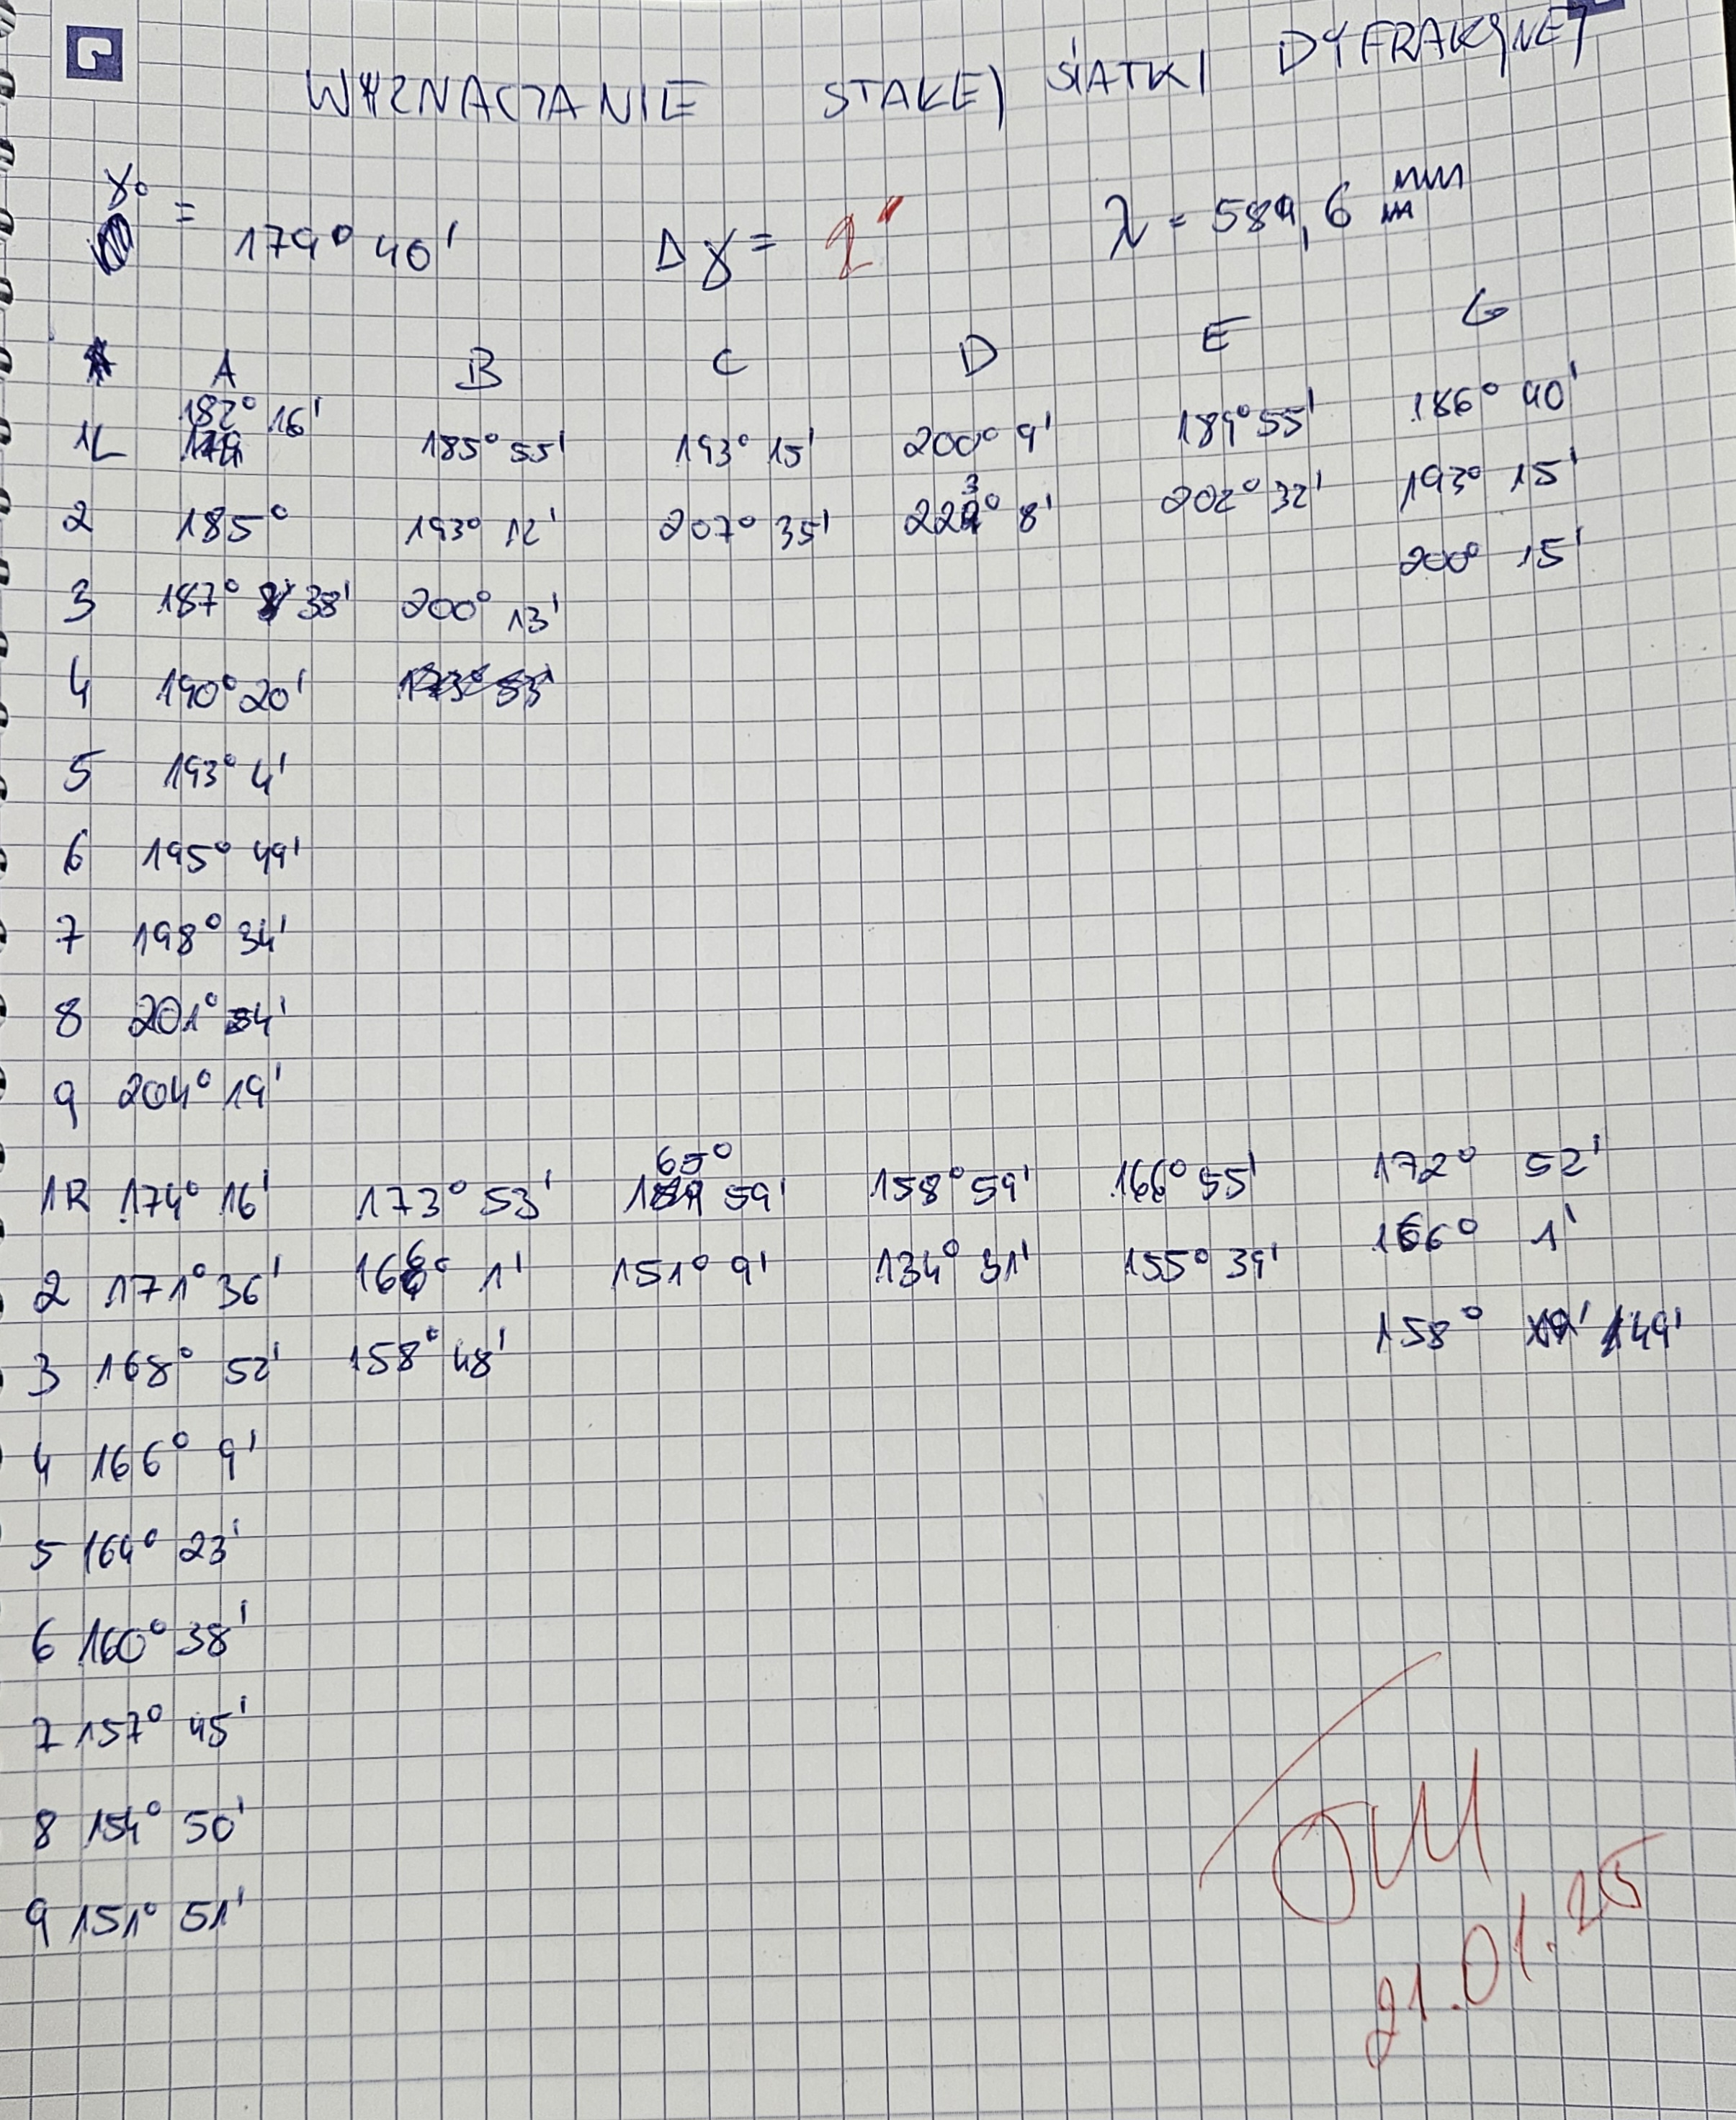
\includegraphics[scale=0.2]{pictures/20250121_124928.jpg}
\end{center}
%section wyniki_pomiarow (end)

\section{Opracowanie wyników}\label{sec:opracowanie_wynikow} % (fold)

\subsection{Obliczenia}\label{sub:obliczenia} % (fold)
\[
	\upsilon_0 = 170,66^{\circ} \qquad \lambda = 589,6 nm
\]

Dla prążka 10 siatki A obliczenia wyglądją następująco
\[
	d_A = \frac{m\lambda}{\text{sin}(\upsilon)}
\]
\[
	\upsilon = \upsilon_0 - \upsilon_{A10} = \left| 170,66^{\circ} - 151,85^{\circ} \right| = 27,81^{\circ}
\]
\[
	d_A = \frac{10 \cdot 598,6}{\text{sin}(27,81^{\circ})} = 12634 nm
\]

\subsubsection{A}\label{sec:a} % (fold)
\begin{center}
	\begin{tabular}{|l|l|l|l|l|l|l|}
		\hline
		$m $ & $\upsilon_{Am} \, [^{\circ}]$ & $\upsilon_{Am} \, [']$ & $\upsilon_{Am} \, [^{\circ}]$ & $\upsilon \, [^{\circ}]$ & $\text{sin}(\upsilon)$ & $d [nm]$ \\ \hline
		10   & 151                           & 51                     & 151.85                        & 27.81                    & 0.46664                & 12634    \\ \hline
		9    & 154                           & 50                     & 154.83                        & 24.83                    & 0.41998                & 12634    \\ \hline
		8    & 157                           & 45                     & 157.75                        & 21.91                    & 0.37325                & 12636    \\ \hline
		7    & 160                           & 38                     & 160.63                        & 19.03                    & 0.32611                & 12655    \\ \hline
		6    & 164                           & 23                     & 164.38                        & 15.28                    & 0.26359                & 13420    \\ \hline
		5    & 166                           & 9                      & 166.15                        & 13.51                    & 0.23372                & 12612    \\ \hline
		4    & 168                           & 52                     & 168.86                        & 10.8                     & 0.18738                & 12586    \\ \hline
		3    & 171                           & 36                     & 171.6                         & 8.06                     & 0.14032                & 12605    \\ \hline
		2    & 174                           & 16                     & 174.26                        & 5.39                     & 0.09410                & 12530    \\ \hline
		1    & ~                             & ~                      & ~                             & ~                        & ~                      & ~        \\ \hline
		1    & 182                           & 16                     & 182.26                        & 2.60                     & 0.04536                & 12997    \\ \hline
		2    & 185                           & ~                      & 185                           & 5.33                     & 0.09294                & 12686    \\ \hline
		3    & 187                           & 38                     & 187.63                        & 7.96                     & 0.13859                & 12762    \\ \hline
		4    & 190                           & 20                     & 190.33                        & 10.66                    & 0.18509                & 12741    \\ \hline
		5    & 193                           & 4                      & 193.06                        & 13.4                     & 0.23174                & 12720    \\ \hline
		6    & 195                           & 49                     & 195.81                        & 16.15                    & 0.27815                & 12718    \\ \hline
		7    & 198                           & 34                     & 198.56                        & 18.9                     & 0.32391                & 12741    \\ \hline
		8    & 201                           & 54                     & 201.9                         & 22.23                    & 0.37837                & 12465    \\ \hline
		9    & 204                           & 19                     & 204.31                        & 24.65                    & 0.41707                & 12722    \\ \hline
	\end{tabular}
\end{center}
% subsubsection A (end)

\subsubsection{B}\label{sec:b} % (fold)
\begin{center}
	\begin{tabular}{|l|l|l|l|l|l|l|}
		\hline
		$m $ & $\upsilon_{Bm} \, [^{\circ}]$ & $\upsilon_{Bm} \, [']$ & $\upsilon_{Bm} \, [^{\circ}]$ & $\upsilon \, [^{\circ}]$ & $\text{sin}(\upsilon)$ & $d [nm]$ \\ \hline
		3    & 158                           & 48                     & 158.8                         & 20.86                    & 0.35619                & 4965.8   \\ \hline
		2    & 166                           & 1                      & 166.0                         & 13.65                    & 0.23599                & 4996.8   \\ \hline
		1    & 173                           & 53                     & 173.8                         & 5.78                     & 0.10076                & 5851.1   \\ \hline
		1    & 185                           & 55                     & 185.9                         & 6.25                     & 0.10886                & 5415.7   \\ \hline
		2    & 193                           & 12                     & 193.2                         & 13.53                    & 0.23401                & 5039.0   \\ \hline
		3    & 200                           & 13                     & 200.2                         & 20.55                    & 0.35102                & 5038.9   \\ \hline
	\end{tabular}
\end{center}
% subsubsection B (end)

\subsubsection{C}\label{sub:c} % (fold)
\begin{center}
	\begin{tabular}{|l|l|l|l|l|l|l|}
		\hline
		$m $ & $\upsilon_{Cm} \, [^{\circ}]$ & $\upsilon_{Cm} \, [']$ & $\upsilon_{Cm} \, [^{\circ}]$ & $\upsilon \, [^{\circ}]$ & $\text{sin}(\upsilon)$ & $d [nm]$ \\ \hline
		2    & 151                           & 9                      & 151.15                        & 28.516                   & 0.47741                & 2469.97  \\ \hline
		1    & 165                           & 59                     & 165.98                        & 13.683                   & 0.23655                & 2492.43  \\ \hline
		1    & 193                           & 15                     & 193.25                        & 13.583                   & 0.23485                & 2510.43  \\ \hline
		2    & 207                           & 35                     & 207.58                        & 27.916                   & 0.46818                & 2518.65  \\ \hline
	\end{tabular}
\end{center}
% subsection C (end)

\subsubsection{D}\label{sec:d} % (fold)
\begin{center}
	\begin{tabular}{|l|l|l|l|l|l|l|}
		\hline
		$m $ & $\upsilon_{Dm} \, [^{\circ}]$ & $\upsilon_{Dm} \, [']$ & $\upsilon_{Dm} \, [^{\circ}]$ & $\upsilon \, [^{\circ}]$ & $\text{sin}(\upsilon)$ & $d [nm]$ \\ \hline
		2    & 134                           & 31                     & 134.51                        & 45.15                    & 0.70895                & 1663.29  \\ \hline
		1    & 158                           & 59                     & 158.98                        & 20.683                   & 0.35320                & 1669.29  \\ \hline
		1    & 200                           & 9                      & 200.15                        & 20.483                   & 0.34993                & 1684.88  \\ \hline
		2    & 223                           & 8                      & 223.13                        & 43.466                   & 0.68793                & 1714.12  \\ \hline
	\end{tabular}
\end{center}
% subsubsection D (end)

\subsubsection{E}\label{sec:e} % (fold)
\begin{center}
	\begin{tabular}{|l|l|l|l|l|l|l|}
		\hline
		$m $ & $\upsilon_{Em} \, [^{\circ}]$ & $\upsilon_{Em} \, [']$ & $\upsilon_{Em} \, [^{\circ}]$ & $\upsilon \, [^{\circ}]$ & $\text{sin}(\upsilon)$ & $d [nm]$ \\ \hline
		2    & 155                           & 39                     & 155.65                        & 24.016                   & 0.40700                & 2897.28  \\ \hline
		1    & 166                           & 55                     & 166.91                        & 12.75                    & 0.22069                & 2671.53  \\ \hline
		1    & 189                           & 55                     & 189.91                        & 10.25                    & 0.17794                & 3313.41  \\ \hline
		2    & 202                           & 32                     & 202.53                        & 22.866                   & 0.38858                & 3034.57  \\ \hline
	\end{tabular}
\end{center}
% subsubsection E (end)

\subsubsection{G}\label{sec:g} % (fold)
\begin{center}
	\begin{tabular}{|l|l|l|l|l|l|l|}
		\hline
		$m $ & $\upsilon_{Gm} \, [^{\circ}]$ & $\upsilon_{Gm} \, [']$ & $\upsilon_{Gm} \, [^{\circ}]$ & $\upsilon \, [^{\circ}]$ & $\text{sin}(\upsilon)$ & $d [nm]$ \\ \hline
		3    & 158                           & 49                     & 158.81                        & 20.85                    & 0.35592                & 4969.61  \\ \hline
		2    & 166                           & 1                      & 166.01                        & 13.65                    & 0.23599                & 4996.81  \\ \hline
		1    & 172                           & 52                     & 172.86                        & 6.799                    & 0.11840                & 4979.56  \\ \hline
		1    & 186                           & 40                     & 186.66                        & 7                        & 0.12186                & 4837.96  \\ \hline
		2    & 193                           & 15                     & 193.25                        & 13.583                   & 0.23485                & 5020.87  \\ \hline
		3    & 200                           & 15                     & 200.25                        & 20.583                   & 0.35156                & 5031.15  \\ \hline
	\end{tabular}
\end{center}
% subsubsection G (end)

% subsection Obliczenia (end)

\subsection{Wyniki}\label{sub:wyniki} % (fold)
\Large
\[
	D_A = 12700 \pm 200 \; nm
\]
\[
	D_B = 5210 \pm 350 \; nm
\]
\[
	D_C = 2500 \pm 20 \; nm
\]
\[
	D_D = 1680 \pm 20 \; nm
\]
\[
	D_E = 2980 \pm 26 \; nm
\]
\[
	D_G = 4970 \pm 70 \; nm
\]
\normalsize
% subsection Wyniki (end)

% section Opracowanie wynikow (end)

\section{Wnioski}\label{sec:wnioski} % (fold)
Różnice pomiędzy wartościami prawdziwymi, a wyliczonymi mogą wynikać z niedokładności przeprowadzonego pomiaru.
% section Wnioski (end)

\end{document}

